
\chapter{\textit{Habitat}: Simulador \textit{Habitat Sim} y \textit{Habitat Lab}}

En este capítulo se describirá en profundidad el simulador utilizado, \textit{Habitat Sim 2.0}, y su librería de Python \textit{Habitat Lab}. Además, se presentarán los principales componentes usados por la librería, detallando su funcionamiento y su uso. Finalmente, se explicará la instalación del simulador y las dependencias necesarias.

\section{\textit{Habitat}}

\textbf{\textit{Habitat}} \cite{habitat19iccv} es una plataforma para el desarrollo de inteligencia artificial con agentes físicos, diseñada con el fin de estandarizar el conjunto de herramientas necesarias para el entrenamiento en entornos hiperrealistas tridimensionales bajo una sola plataforma unificada e integrada.

Esta plataforma pretende resolver algunos de los problemas tradicionales que afectan a otros simuladores, impidiendo la generalización y comparación de resultados experimentales \cite{habitat19iccv}:
\begin{itemize}
	\item La dependencia entre componentes (como simuladores funcionando únicamente con conjuntos de datos o tareas especificas), dificultando el trabajo al necesitar varias herramientas.
	\item Los parámetros fijos (como las acciones disponibles, los sensores...), dificultando la comparativa de resultados.
	\item El rendimiento subóptimo de los simuladores (tanto en renderizado como en físicas), dificultando el entrenamiento de agentes a gran escala. 
\end{itemize}

La plataforma \textit{Habitat} cuenta con dos componentes principales \cite{habitat19iccv}:
\begin{itemize}
	\item \textbf{\textit{Habitat Sim}:} Un simulador 3D modificable con agentes configurables, diversos sensores y manejo de conjuntos de datos 3D genéricos (con soporte de fábrica para conjuntos como \textit{Matterport3D} o \textit{Gibson}).
	\item \textbf{\textit{Habitat Lab}:} Una librería modular de alto nivel desarrollada para Python, con el fin de facilitar el desarrollo de agentes físicos en \textit{Habitat Sim}, ofreciendo herramientas para la definición, configuración, entrenamiento y evaluación de éstos.
\end{itemize}

\subsection{Simulador \textit{Habitat Sim}}

\textbf{\textit{Habitat Sim}} \cite{habitat19iccv} es un simulador 3D ampliable, diseñado para el entrenamiento de agentes físicos en entornos hiperrealistas. Este simulador se encarga de representar escenarios tridimensionales en formatos estandarizados y de simular agentes físicos, tanto sensores como movimiento. 

Este simulador fue diseñado con el propósito de solventar los problemas descritos previamente, siendo algunos de sus objetivos principales:

\begin{itemize}
	\item \textbf{Soporte genérico a conjuntos de datos:} \textit{Habitat Sim} es capaz de reconstruir y simular conjuntos de datos genéricos independientemente de su origen, usando un formato uniforme y estandarizado como son los \textit{scene graphs} \cite{DBLP:journals/corr/abs-2104-01111} (representaciones estructuradas de los escenarios). Esta estandarización permite al simulador trabajar de forma consistente con cualquier conjunto de datos.
	\item \textbf{Modularidad:} El simulador está diseñado ofreciendo \textit{APIs} de todos sus componentes, permitiendo la ampliación del simulador con nuevos sensores, escenarios, tareas...
	\item \textbf{Rendimiento:} \textit{Habitat Sim} está implementado en C++ usando la librería \textit{Magnum Graphics} como \textit{middleware} para el procesamiento de la imagen. Además, la tubería de creación y renderizado de imágenes está optimizada para evitar la repetición de procesos, siendo capaz de generar todas las imágenes de cada instante en una única pasada.
	
	Todo ésto permite al simulador generar miles de \textit{frames} por segundo, siendo este valor al menos un orden de magnitud superior al que ofrecen otros simuladores como \textbf{Gibson} \cite{xiazamirhe2018gibsonenv} o \textbf{MINOS} \cite{DBLP:journals/corr/abs-1712-03931}. Esta velocidad mueve el cuello de botella de la simulación al entrenamiento del agente, permitiendo entrenamientos más profundos en menos tiempo.
\end{itemize}

\textbf{\textit{Habitat 2.0}} \cite{szot2021habitat} es una versión posterior de \textit{Habitat Sim} lanzada en Junio de 2021, diseñada con el fin de ser capaz de simular entornos interactivos con físicas complejas (frente a las simulaciones de físicas simples de \textit{Habitat Sim}) y centrada en permitir la creación y evaluación de agentes físicos asistentes. Las principales características ofrecidas son:

\begin{itemize}
	\item \textbf{Simulador \textit{Habitat 2.0}:} Una segunda versión del simulador \textit{Habitat Lab} con capacidad para simular movimientos y físicas de objetos rígidos (como puertas, cajones...), robots articulados, cinemáticas, dinámicas...
	
El rendimiento del simulador es superior al de \textit{Habitat Sim}, especialmente durante la simulación de físicas. Además, el rendimiento escala notablemente, pudiendo trabajar de forma distribuida. 
	
	\item \textbf{Conjunto de datos \textit{ReplicaCAD}:} \textit{ReplicaCAD} es un conjunto de datos creado a partir del conjunto \textit{Replica} \cite{DBLP:journals/corr/abs-1906-05797}. Este conjunto de datos está diseñado para aprovechar las capacidades del nuevo simulador y pensado para evaluación de tareas de reorganización de elementos, implementando objetos articulados e interactivos.
	
	\item \textbf{\textit{Home Assistant Benchmark (HAB)}:} Un \textit{benchmark} implementando un conjunto de tareas típicas para robots asistentes (como limpiar un cuarto o preparar una mesa), diseñado para evaluar el rendimiento de estos agentes de forma estandarizada.
\end{itemize}

\subsection{Librería \textit{Habitat Lab}}

\textit{Habitat Lab} (originalmente conocido como \textit{Habitat-API}) \cite{habitat19iccv} es una librería modular de alto nivel desarrollada para \textit{Python}, con el fin de facilitar el uso de \textit{Habitat Sim} y el desarrollo de agentes físicos. El principal objetivo de la librería es permitir a los usuarios:

\begin{itemize}
	\item \textbf{Definir tareas para agentes físicos}: Se ofrecen tareas típicas (como navegación, seguimiento de orden, búsqueda de objetos...) y \textit{APIs} para desarrollar tareas propias.
	\item \textbf{Configurar agentes físicos:} Se permite modificar al agente físico ajustando su forma  física, los sensores disponibles, las acciones posibles...
	\item \textbf{Entrenar agentes físicos:} Se ofrece soporte para técnicas clásicas (como \textit{SLAM}) además de entrenamiento por refuerzo y entrenamiento por imitación.
	\item \textbf{Evaluar agentes físicos:} Se ofrecen métricas estándares \cite{DBLP:journals/corr/abs-1807-06757} usadas para evaluar el rendimiento de los agentes.
\end{itemize}

Además, la librería opcionalmente ofrece \textit{Habitat Baselines}, un conjunto de ejemplos y ampliaciones a \textit{Habitat Lab}. Entre estas ampliaciones se incluyen diversas utilidades para facilitar el desarrollo, agentes prediseñados y ejemplos para entender el funcionamiento del simulador y la librería.


\section{Conceptos principales de \textit{Habitat}}

La arquitectura de \textit{Habitat} (y, especialmente, la de la librería \textit{Habitat Lab}) gira principalmente en torno a tres conceptos principales, como se puede ver en la Figura \ref{fig:chap4-habitat}:

\begin{figure}[h]
    \centering
    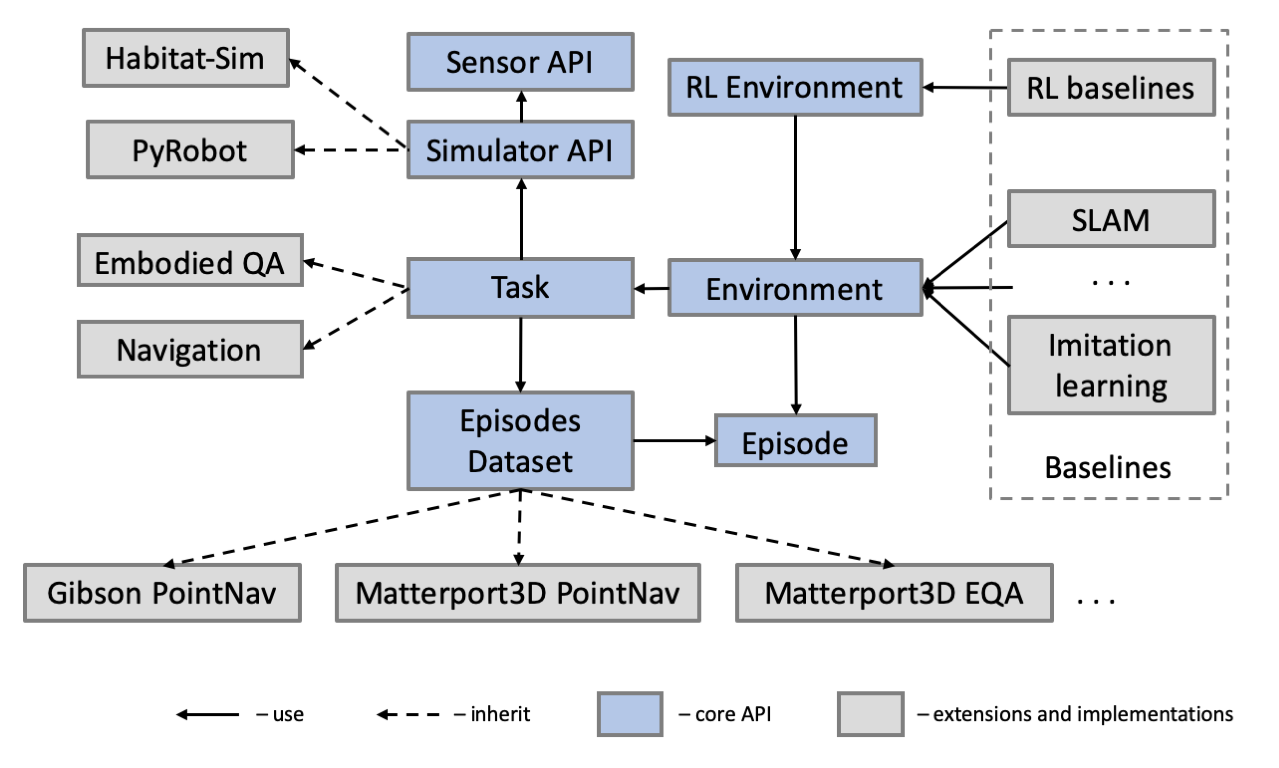
\includegraphics[width=\textwidth]{imagenes/cap4/habitat_lab_structure.png}
    \caption{Arquitectura de \textit{Habitat Lab} \cite{habitat19iccv}.}
    \label{fig:chap4-habitat}
\end{figure}

\begin{enumerate}
	\item \textbf{Tarea (\textit{Task)}:} El problema concreto a resolver por el agente, gestiona los objetivos y el éxito de la tarea usando métricas del simulador.
	\item \textbf{Episodio (\textit{Episode)}:} Especificación del episodio a realizar, conteniendo información como la posición y ángulo iniciales del agente, posición de la meta...
	\item \textbf{Entorno (\textit{Environment)}:} Concepto principal del simulador, abstrae toda la información necesaria para permitir el trabajo con el simulador y el agente físico.
\end{enumerate}

Ahora bien, la documentación oficial del simulador es pobre y ofrece poca información sobre los conceptos y, especialmente, sobre su uso. Además, hay otros conceptos (como entrenadores, ficheros de configuración...) de igual relevancia e importancia para el uso del simulador que no reciben ninguna explicación. 

Por tanto, en esta sección se busca explicar en detalle los conceptos principales necesarios para trabajar con \textit{Habitat}, detallando sus características y su uso.

\subsection{Entornos}

Un \textbf{entorno (\textit{environment})} es el concepto principal de \textit{Habitat Lab}. El entorno se encarga de abstraer las principales tareas necesarias para el trabajo con agentes físicos, siendo las principales tareas que realiza:

\begin{itemize}
	\item \textbf{Carga y manejo del conjunto de datos:} El entorno se encarga de la lectura y carga de los ficheros, y de la conversión de los escenarios al formato de \textit{scene graph}. 
	\item \textbf{Control de las métricas y los objetivos de la tarea:} El entorno se encarga de la interacción con el simulador para el control de los objetivos y las métricas de la tarea. Además, se encarga de detener los episodios cuando se cumplen los objetivos.
	\item \textbf{Generación y manejo de los episodios:} El entorno genera la lista de episodios a partir del conjunto de datos y de la tarea a realizar. Además, se encarga de ordenar los episodios de forma óptima (juntando los episodios que se realizan en un mismo escenario) para agilizar el proceso.
	\item \textbf{Control del agente físico:} El entorno interactúa con el simulador en ambos sentidos, leyendo los sensores del agente físico y devolviendole la acción realizada para simular los resultados.
\end{itemize}

Por defecto, \textit{Habitat Lab} ofrece dos tipos de entornos, a partir de los cuales se puede derivar cualquier entorno necesario.

\subsubsection{\textit{Env}}

\textbf{\textit{Env}} es el simulador básico ofrecido por \textit{Habitat}, usado principalmente para agentes sin aprendizaje y para la evaluación de agentes entrenados, implementando todas las características descritas previamente. El entorno ofrece dos métodos básicos, usados para controlar la simulación:

\begin{itemize}
	\item \textbf{reset():} Este método se encarga de preparar el entorno para el comienzo de un episodio, cargando el escenario y configurándolo para el episodio actual. Además, devuelve las primeras observaciones que recibe el agente con el sensor, para poder actuar a partir de ellas.
	\item \textbf{step(acción):} Dada una acción como argumento, el entorno aplica la acción al agente físico y devuelve las nuevas percepciones del agente a través de sus sensores.
\end{itemize}

Cualquier entorno personalizado que se quiera crear debe ser una subclase de \textit{Env} (al ofrecer toda la funcionalidad básica).

\subsubsection{\textit{RLEnv}}

\textbf{\textit{RLEnv}} es la principal subclase de \textit{Env} disponible, ofreciendo capacidades adicionales al entorno para permitir el entrenamiento usando aprendizaje por refuerzo. Además de los métodos anteriores, incluye varios más que deben ser implementados para su funcionamiento:

\begin{itemize}
	\item \textbf{get{\_}reward(observaciones):} A partir de las observaciones del agente, calcula una recompensa o penalización para éste. En general, el procesamiento de recompensas se implementa directamente en el entorno a través de este método.
	
	\item \textbf{get{\_}reward{\_}range():} Este método únicamente devuelve los límites de la recompensa (el rango $[min, max]$ en el que se encuentra).
	
	\item \textbf{get{\_}done(observaciones):} A partir de las observaciones del agente, calcula si el episodio ha acabado (ya sea de forma satisfactoria o fallida). En este método se implementan comprobaciones como colisiones u otras condiciones de parada.
	
	\item \textbf{get{\_}info(observaciones):} Devuelve información respecto al entorno a partir de la última observación. Es típico devolver información de sensores o métricas con este método. 
\end{itemize}

Por defecto, \textit{RLEnv} no implementa los métodos descritos previamente, por lo que es necesario realizar un entorno personalizado para el entrenamiento. Ahora bien, \textit{Habitat Baselines} ofrece \textit{NavRLEnv}, una implementación básica de entorno pensado para problemas de navegación a objetivo que sirve como punto de partida para otras implementaciones más complejas.

En este trabajo, se ha implementado un entorno personalizado (\textit{ReactiveNavigationEnv}) como subclase de \textit{NavRLEnv}, con definiciones propias de los métodos previos para usar el sistema de recompensas basado en potenciales propuesto (descrito en más detalle en el Capítulo 5).

\subsection{Tareas}

Una \textbf{tarea (\textit{embodied task})} es un contenedor de la información necesaria para que el simulador pueda definir y trabajar con una tarea. Concretamente, contiene información sobre:

\begin{itemize}
	\item El \textbf{espacio de acciones} disponible.
	\item Los \textbf{sensores} disponibles para el agente.
	\item Las \textbf{métricas} a utilizar para valorar al agente.
	\item El \textbf{simulador} sobre el que se va a trabajar.
\end{itemize}

La clase \textit{EmbodiedTask} implementa los métodos básicos para la definición de tareas, y todas las tareas diseñadas deben heredar de esta. Ahora bien, \textit{Habitat Lab} ofrece varias tareas típicas por defecto:

\begin{itemize}
	\item \textbf{\textit{NavigationTask} (navegación a meta / objetivo):} El objetivo del agente es alcanzar una posición, dada sus coordenadas. La mayoría de tareas que incluyen navegación se definen como subclases de esta tarea. Es la tarea más típica, y la que se busca resolver en este trabajo.
	
	\item \textbf{\textit{ObjectNavigationTask} (navegación a objeto):} Una variante de \textit{NavigationTask}, en la que el agente debe desplazarse hasta un objeto concreto localizado en el entorno.
	
	\item \textbf{\textit{VLNTask / Vision and Language Navigation Task} (navegación con visión y lenguaje):} Una variante de la \textit{NavigationTask}, en la que el agente debe alcanzar una meta siguiendo instrucciones expresadas en lenguaje natural.
	
	\item \textbf{\textit{EQATask / Embodied Question Answering Task} (respuesta física a preguntas) \cite{eqa_matterport}:} El agente recibe una pregunta en lenguaje natural (como, por ejemplo, \textit{"¿De qué color es el coche aparcado el garaje?"}) y debe explorar el entorno para ser capaz de responder.
	
	\item \textbf{\textit{RearrangeTask} (re-organización):} Tareas introducidas con \textit{Habitat 2.0}, \textit{RearrangeTask} es una tarea genérica introducida para ofrecer soporte a tareas que necesitan agentes con articulaciones móviles. Actualmente existen dos tareas de reorganización, \textbf{\textit{RearrangePickTask}} (agarrar un objeto determinado del entorno) y \textbf{\textit{RearrangeReachTask}} (alcanzar un objeto determinado del entorno).
	
\end{itemize}

Estas tareas se instancian a partir del fichero de configuración, como se verá posteriormente. Es importante destacar que no todos los sensores y métricas son compatibles con todas las tareas. Algunos de ellos han sido diseñados para tareas específicas, y no pueden ser usados fuera de éstas.

\subsection{Episodios}

Un \textbf{episodio (\textit{episode})} es una especificación de una instancia específica de un agente en un escenario realizando una tarea, incluyendo la información relativa al estado inicial y a la meta a cumplir. Por defecto, un episodio (\textit{Episode)} contiene información sobre:

\begin{itemize}
	\item \textbf{Posición} y \textbf{rotación} inicial del agente.
	\item \textbf{Escenario} en el que se realiza el episodio.
\end{itemize}

Al igual que con las tareas, la clase \textit{Episode} es una clase genérica que implementa únicamente los métodos básicos y de la que se deben derivar las definiciones de episodios, existiendo subclases de episodios para cada tarea específica:

\begin{itemize}
	\item \textbf{\textit{NavigationEpisode} (episodio de navegación):} Incluye información adicional sobre las coordenadas de la meta y la ruta más corta desde la posición inicial hasta la meta. 
	
	\item \textbf{\textit{ObjectGoalNavigationEpisode} (episodio de navegación a objeto):} Incluye información adicional sobre las coordenadas del objeto a encontrar y la ruta más corta desde la posición inicial hasta el objeto.
	
	\item \textbf{\textit{VLNEpisode} (episodio de navegación con visión y lenguaje):} Incluye información adicional sobre las coordenadas de la meta y las instrucciones en lenguaje natural proporcionadas al agente.

	\item \textbf{\textit{EQAEpisode} (episodio de respuesta física a preguntas):} Incluye información adicional sobre la pregunta y la respuesta esperada.
	
	\item \textbf{\textit{RearrangeEpisode} (episodio de reorganización):} Incluye información adicional sobre las partes articuladas del escenario y los objetos a alcanzar o agarrar. 	
	
\end{itemize}

Los episodios son creados y gestionados automáticamente por los conjuntos de datos, como se verá a continuación.

\subsection{Conjuntos de datos}

Un \textbf{conjunto de datos \textit{(dataset)}} es un contenedor y gestor de episodios a realizar, encargándose de:

\begin{itemize}
	\item \textbf{Cargar los escenarios desde memoria}, convirtiendo los \textit{meshes} (información sobre la estructura tridimensional del escenario) al formato de \textit{state graph} esperado.
	\item \textbf{Crear los episodios} automáticamente a partir de la información del conjunto de datos.
	\item \textbf{Gestionar la iteración de episodios}, ordenándolos de forma que se reduzcan las lecturas de ficheros.
	\item Permitir al usuario \textbf{filtrar los episodios} en base a criterios especificados.
\end{itemize}

De forma similar a las tareas y los episodios, existe una clase base \textit{Dataset} que implementa toda la lógica necesaria, existiendo subclases para cada tipo de tarea:

\begin{itemize}
\item \textbf{\textbf{\textit{PointNavDatasetV1}}} para \textit{NavigationTask} y \textit{NavigationEpisode}.
\item \textbf{\textit{ObjectNavDatasetV1}} para \textit{ObjectNavigationTask} y \textit{ObjectGoalNavigationEpisode}
\item \textbf{\textit{VLNDatasetV1}} para \textit{VLNTask} y \textit{VLNEpisode}.
\item \textbf{\textit{Matterport3DDatasetV1}} para \textit{EQATask} y \textit{EQAEpisode}. Este conjunto de datos funciona exclusivamente con \textit{Matterport3D}.
\item \textbf{\textit{RearrangeDatasetV0}} para tareas de reorganización (\textit{RearrangePickTask} y \textit{RearrangeReachTask}) y \textit{RearrangeEpisode}.
\end{itemize}

\textit{Habitat} ofrece por defecto soporte a cuatro conjuntos de datos. Además, espera que éstos (y cualquier otro conjunto de datos personalizado que se use) siga una estructura específica. Ambos puntos serán detallados a continuación.

\subsubsection{Conjuntos de datos disponibles}

La primera versión de \textit{Habitat Lab} ofrece por defecto soporte a \textbf{dos} conjuntos de datos típicos para el entrenamiento de agentes físicos en interiores:

\begin{itemize}
	\item \textbf{\textit{Matterport3D} \cite{Matterport3D}:} \textit{Matterport3D} es un conjunto de datos de gran escala formado por \textbf{199,400} imágenes \textit{RGB-D} (imágenes obtenidas por cámaras de color y profundidad) tomadas por una cámara \textit{Matterport}, formando un total de \textbf{10,800} vistas panorámicas de 90 edificios (incluyendo edificios públicos, oficinas e interiores de viviendas).
	
	Este conjunto de datos incluye información sobre:
	\begin{itemize}
		\item Reconstrucciones 3D del escenario, con texturas a partir de las panorámicas.
		\item Panorámicas de color (\textit{RGB}).
		\item Panorámicas de profundidad.
		\item Anotaciones semánticas (tanto a nivel de objetos como de regiones de los escenarios)
		\item \textit{Normales} de las superficies.
	\end{itemize}
	
	Se puede observar un ejemplo de un escenario en la Figura \ref{fig:chap4-matterport}.
	
	\begin{figure}[h]
    \centering
    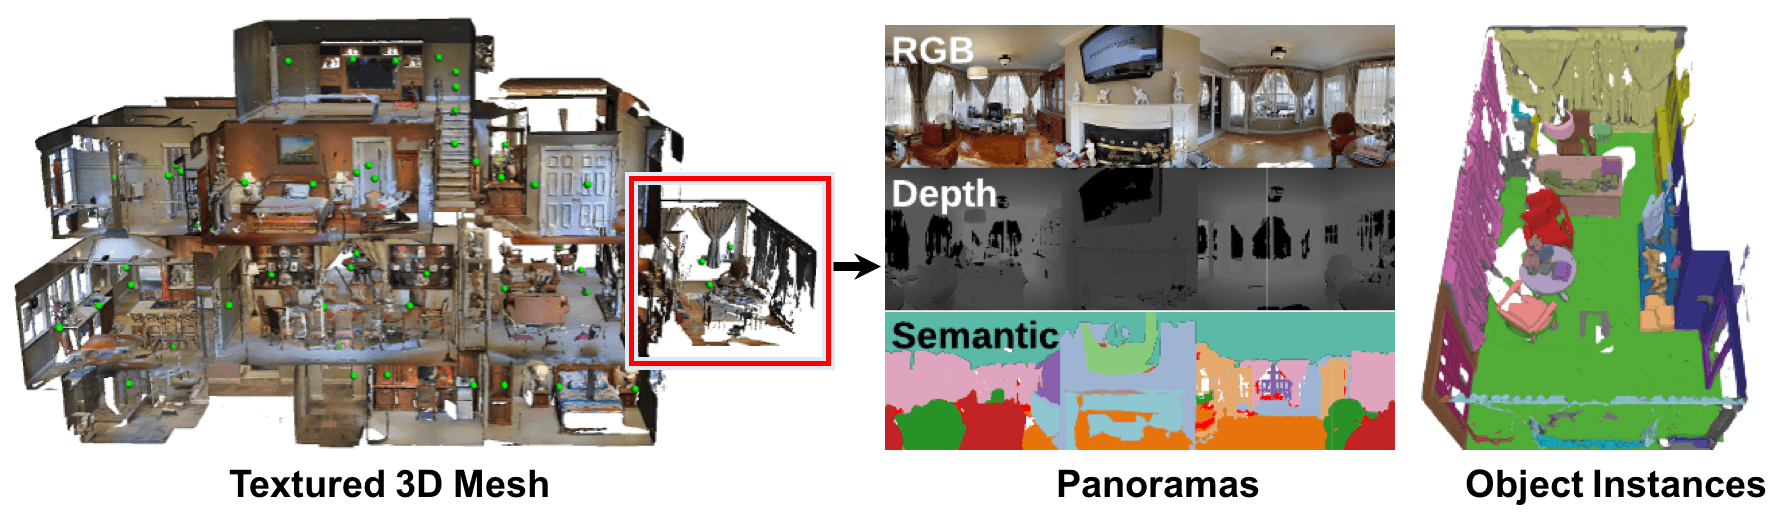
\includegraphics[width=\textwidth]{imagenes/cap4/matterport.png}
    \caption{Modelos 3D de \textit{Matterport3D}, y panorámicas asociadas \cite{Matterport3D}.}
    \label{fig:chap4-matterport}
\end{figure}
	
	\item \textbf{\textit{Gibson} \cite{xiazamirhe2018gibsonenv}:}	\textit{Gibson} es un conjunto de datos originalmente diseñado para el simulador \textit{Gibson}, generado a partir de escaneo 3D y reconstrucción de espacios del interior de edificios. El conjunto de datos cuenta con \textbf{572} edificios, llegando a un total de \textbf{1447} plantas con una superficie total de \textbf{211} kilómetros cuadrados.
	
	Este conjunto de datos incluye información sobre:
	\item Reconstrucciones 3D del escenario, con texturas a partir de las panorámicas.
		\item Panorámicas de color (\textit{RGB}).
		\item Panorámicas de profundidad.
		\item \textit{Normales} de las superficies.
		
	Además, una fracción de los escenarios incluyen anotaciones semánticas sobre los objetos contenidos. Se puede ver un ejemplo de un escenario en la Figura \ref{fig:chap4-gibson}.

\begin{figure}[h]
    \centering
    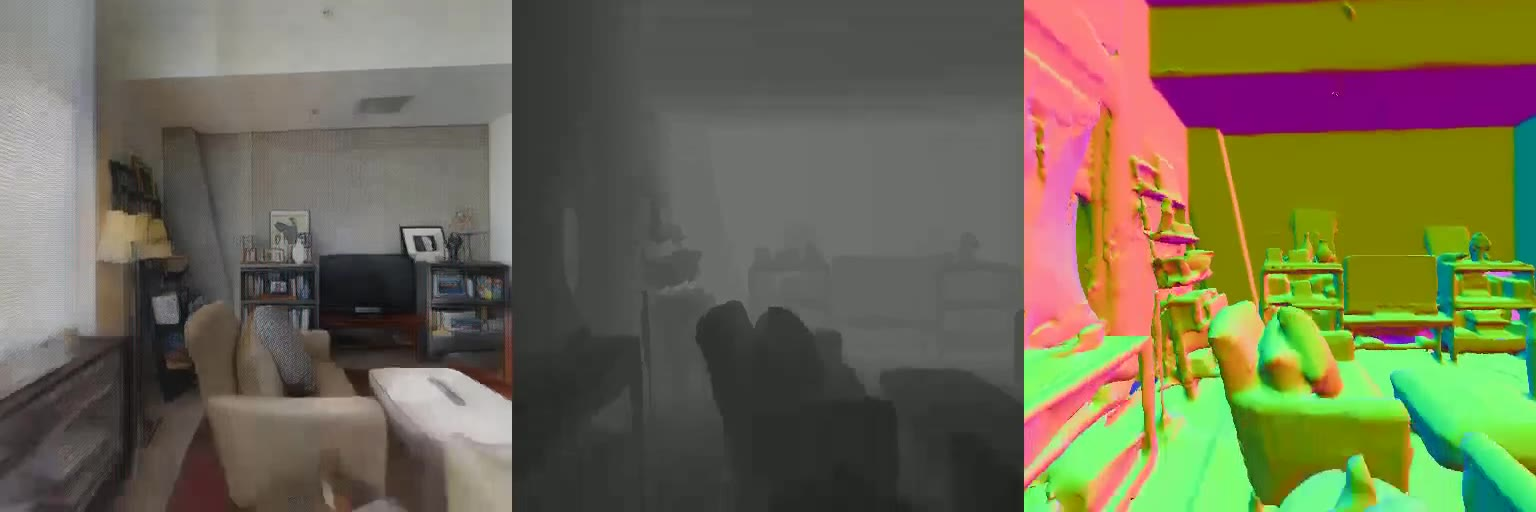
\includegraphics[width=\textwidth]{imagenes/cap4/gibson.jpg}
    \caption{Imagen de color (izquierda), profundidad (centro) y normales (derecha) de un escenario de \textit{Gibson} \cite{xiazamirhe2018gibsonenv}.}
    \label{fig:chap4-gibson}
\end{figure}

\end{itemize}

En general, tanto \textit{Matterport3D} como \textit{Gibson} son conjuntos de datos extensos con información similar, pudiendo cumplir las mismas funciones. Ahora bien, \textit{Gibson} se considera un conjunto más \textit{"fácil"} para el entrenamiento de agentes físicos \cite{habitat19iccv}, al estar formado por escenarios más pequeños.

\textit{Habitat 2.0} añadió soporte a \textbf{dos} conjuntos de datos adicionales por defecto:
\begin{itemize}
	\item \textbf{\textit{ReplicaCAD} \cite{szot2021habitat}:} \textit{ReplicaCAD} es una recreación del conjunto de datos \textit{Replica} \cite{DBLP:journals/corr/abs-1906-05797}, adaptado para el motor de físicas de \textit{Habitat 2.0}. Se puede ver un ejemplo de esta recreación en la Figura \ref{fig:chap4-replicaCAD}.
	
	El conjunto de datos cuenta con \textbf{6} cuartos (teniendo cada cuarto \textbf{5} variaciones y ruido añadido proceduralmente), donde todos los objetos incluyen simulaciones físicas y anotaciones semánticas.
	
	Este conjunto de datos está diseñado expresamente para tareas de reorganización, no estando preparado para otras tareas como navegación.
	
\begin{figure}[h]
    \centering
    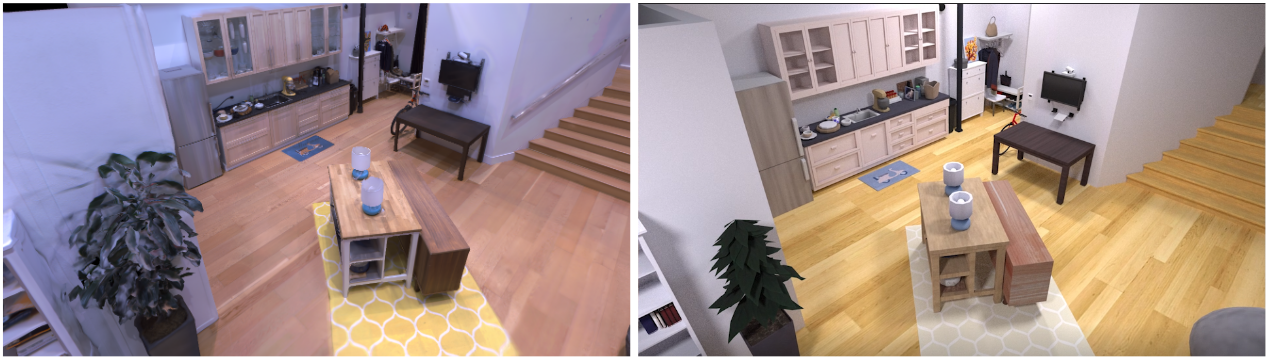
\includegraphics[width=\textwidth]{imagenes/cap4/replicaCAD.png}
    \caption{Escenario original de \textit{Replica} (izquierda) y escenario reconstruido de \textit{ReplicaCAD} (derecha) \cite{szot2021habitat}.}
    \label{fig:chap4-replicaCAD}
\end{figure}	
	
	\item \textbf{\textit{Habitat-Matterport 3D Research Dataset} \cite{habitatmp3d}:} \textit{Habitat-Matterport 3D Research Dataset} (también conocido como \textit{HM3D}) es un conjunto de datos diseñado por el \textit{Facebook AI Research}, generado a partir de imágenes tomadas con cámaras \textit{Matterport}.
	
	Actualmente cuenta con \textbf{1000} escenarios 3D realizados con imágenes de alta resolución de edificios residenciales, comerciales, públicos... Esto lo hace el conjunto de datos más grande actualmente, con alrededor de \textbf{365} kilómetros cuadrados de superficie.
	
	El conjunto de datos ofrece la siguiente información:
	
	\begin{itemize}
		\item Reconstrucciones 3D del escenario, con texturas a partir de las panorámicas.
		\item Panorámicas de color (\textit{RGB}).
		\item Panorámicas de profundidad.
		\item Anotaciones de metadatos de cada escena (incluyendo información como la valoración, el numero de pisos y cuartos, la cantidad de ruido en el escenario...)
	\end{itemize}
	
	Se puede observar un ejemplo de un escenario con la información en la Figura \ref{fig:chap4-hm3d}.	
	
	\begin{figure}[h]
    \centering
    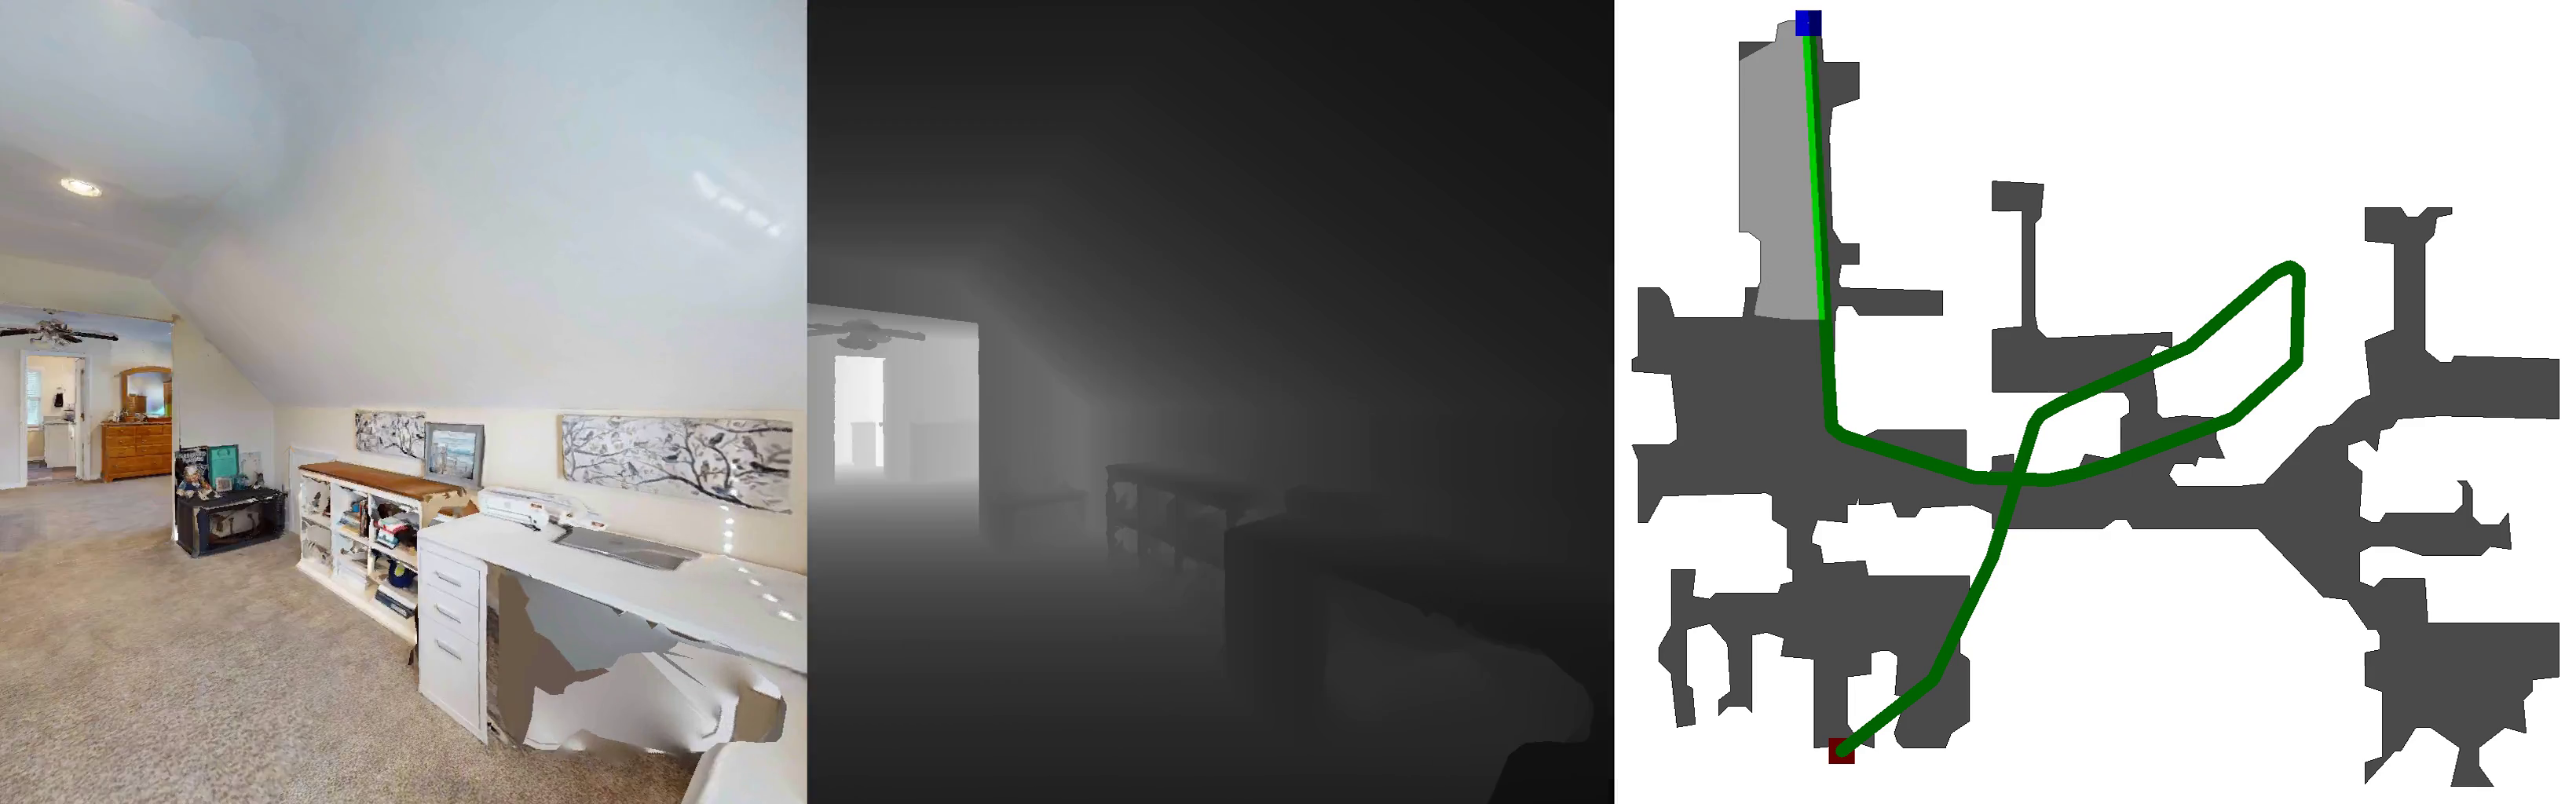
\includegraphics[width=\textwidth]{imagenes/cap4/hm3d.png}
    \caption{Imagen de color (izquierda), profundidad (centro) y mapa (derecha) de una escena de \textit{HM3D} \cite{habitatmp3d}.}
    \label{fig:chap4-hm3d}
\end{figure}	
\end{itemize}

El conjunto \textit{HM3D} ofrece características y dificultad similar a \textit{Matterport3D} y \textit{Gibson}, siendo su principal diferencia la cantidad de escenarios disponibles.

\subsubsection{Estructura de los conjuntos de datos}

Para trabajar con conjuntos de datos, \textit{Habitat} espera que se siga una estructura concreta en el árbol de directorios, como se puede ver en la Figura \ref{fig:tree}.

Especificamente, se espera una carpeta base \textit{data} (o un enlace simbólico a la misma) en el mismo directorio que el fichero ejecutable, que debe tener en su interior a su vez dos carpetas:

\begin{figure}[h]
\centering
\begin{forest}
  for tree={
    font=\ttfamily,
    grow'=0,
    child anchor=west,
    parent anchor=south,
    anchor=west,
    calign=first,
    edge path={
      \noexpand\path [draw, \forestoption{edge}]
      (!u.south west) +(7.5pt,0) |- node[fill,inner sep=1.25pt] {} (.child anchor)\forestoption{edge label};
    },
    before typesetting nodes={
      if n=1
        {insert before={[,phantom]}}
        {}
    },
    fit=band,
    before computing xy={l=15pt},
  }
[data
  [scene{\_}datasets
    [(nombre del dataset 1)]
    [...]
    [(nombre del dataset n)]
  ]
  [datasets
    [(tarea 1)
    	[(nombre del dataset 1)
    		[(version del dataset)
    			[train]
    			[val]
    		]
    	]
    	[...]
    	[(nombre del dataset n)]
    ]
    [...]
    [(tarea n)]
  ]
]
\end{forest}
\caption{Ejemplo de árbol de directorios de la carpeta \textit{data}.}
\label{fig:tree}
\end{figure}

\begin{itemize}
	\item \textbf{\textit{scene{\_}datasets}:} Esta carpeta contiene los modelos 3D de las escenas de cada conjunto de datos, estando cada conjunto contenido en una carpeta con su nombre. Los escenarios en general se encuentran en formato \textit{.glb}, aunque pueden usarse otros.
	\item \textbf{\textit{datasets}:} Esta carpeta contiene, para cada tarea, la definición de todos los escenarios (posición inicial, meta...) para cada conjunto de datos. \textit{Habitat Lab} ofrece estos conjuntos, pudiendo descargarse desde el repositorio de \textit{GitHub}. 
\end{itemize}

\subsection{Acciones}

Una \textbf{acción} \textit{(action)} representa una acción que el agente puede realizar en el entorno mientras resuelve una tarea.

Las acciones derivan de la clase base \textit{SimulatorTaskAction}. Cada tarea incluye un conjunto de acciones posibles, siendo las principales acciones relacionadas con navegación las siguientes:

\begin{itemize}
	\item \textbf{\textit{MOVE{\_}FORWARD}:} Mueve el agente hacia adelante. Por defecto, el agente avanza $0.25m$.
	\item \textbf{\textit{TURN{\_}RIGHT / TURN{\_}LEFT}:} Gira al agente sobre sí mismo hacia la derecha o la izquierda respectivamente. Por defecto, el agente rota $10$ grados.
	\item \textbf{\textit{LOOK{\_}UP / LOOK{\_}DOWN}:} Mueve el ángulo de visión del agente hacia arriba o hacia abajo respectivamente. Por defecto, el ángulo se mueve $15$ grados.
	\item \textbf{\textit{TELEPORT}:} Teletransporta al agente a las coordenadas indicadas.
	\item \textbf{\textit{VELOCITY{\_}CONTROL}:} Ajusta la velocidad lineal y angular del agente a la indicada.
	\item \textbf{\textit{STOP}:} Finaliza el episodio actual, evaluando si ha sido un éxito o no dependiendo de las métricas usadas. Esta acción es importante para evaluar el rendimiento de los agentes en tareas de navegación \cite{DBLP:journals/corr/abs-1807-06757}.
\end{itemize}

Existen otras acciones relacionadas con otras tareas (como \textit{VLN}, \textit{EQA} o \textit{reorganización}) que no han sido mencionadas al no ser relevantes para el problema de navegación a resolver.

\subsection{Sensores}

Un \textbf{sensor} proporciona información del entorno al agente. Esta información es recibida tras cada paso de simulación realizado (siendo el valor devuelto por el método \textit{step} de los entornos).

La clase \textit{Sensor} implementa la funcionalidad básica, existiendo gran cantidad de sensores para diversas tareas. A continuación se describen algunos de los sensores más importantes para navegación:

\begin{itemize}
	\item \textbf{Cámaras:} Las cámaras ofrecen información visual (imágenes) del entorno, devuelta en forma de matriz de valores numéricos. Por defecto, las cámaras apuntan hacia el frente del agente con un ángulo de visión de 90 grados. Existen tres tipos básicos de cámaras disponibles:
	\begin{itemize}
		\item \textbf{Cámara de color (\textit{RGB{\_}SENSOR}):} Devuelve una imagen en color (siguiendo el formato RGB).
		\item \textbf{Cámara de profundidad (\textit{DEPTH{\_}SENSOR}):} Devuelve una imagen en escala de grises representando la profundidad percibida por la cámara. Los valores de esta imagen se representan en forma de números reales en el rango $[0, 1]$ siendo $0.0$ lo más cercano a la cámara y $1.0$ lo más lejano.
		\item \textbf{Cámara semántica (\textit{SEMANTIC{\_}SENSOR}):} Devuelve una imagen seccionada en categorías semánticas (como suelo, techo...). Cada categoría semántica tiene un color asociado. Esta cámara solo puede usarse en conjuntos de datos compatibles con anotaciones semánticas. 
	\end{itemize}
	
	Se puede ver un ejemplo de la misma escena vista desde los tres tipos de cámaras en la Figura \ref{fig:chap4-cameras}.
	
	\begin{figure}[h]
    \centering
    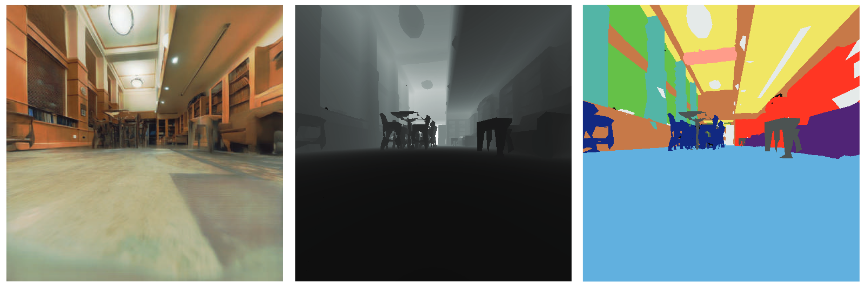
\includegraphics[width=\textwidth]{imagenes/cap4/cameras.png}
    \caption{Imagen de color (izquierda), profundidad (centro) y semántica (derecha) de una escena de \textit{Gibson} \cite{xiazamirhe2018gibsonenv}.}
    \label{fig:chap4-cameras}
\end{figure}		

	\item \textbf{Indicadores de posición:} Los indicadores de posición dan información al agente sobre su propia posición o la de la meta. Estos sensores son exclusivos de tareas de navegación, siendo los principales:
	\begin{itemize}
	\item \textbf{\textit{GPS (GPS{\_}SENSOR)}:} Indica las coordenadas actuales del agente.
	\item \textbf{Brújula \textit{(COMPASS{\_}SENSOR}):} Indica la orientación actual del agente.
	\item \textbf{Meta \textit{(POINTGOAL{\_}SENSOR)}:} Indica las coordenadas de la meta.
	\item \textbf{Combinado \textit{(POINTGOAL{\_}WITH{\_}GPS{\_}COMPASS{\_}SENSOR)}:} Una combinación de los tres sensores anteriores, indicando las coordenadas de agente y meta y el ángulo del agente. Además, indica la distancia del agente a la meta.
	\item \textbf{Proximidad \textit{(PROXIMITY{\_}SENSOR)}:} Indica la distancia en metros del obstáculo más cercano al agente.
	\end{itemize}
\end{itemize}

\subsection{Métricas}

Una \textbf{métrica} \textit{(measure)} indica información sobre la tarea que se está realizando. Esta información no está disponible para el agente, sino que se usa para evaluar el éxito de los episodios y para obtener estadísticas del proceso.

La clase \textit{Measure} implementa la funcionalidad básica de las métricas, de la que se debe derivar cualquier otra métrica definida. Además, las métricas se definen para tareas específicas, no pudiendo usarse métricas de una tarea en otra distinta. Las principales métricas usadas en navegación son:

\begin{itemize}
	\item \textbf{Distancia a la meta \textit{(DISTANCE{\_}TO{\_}GOAL)}:} Indica la distancia actual en metros entre el agente y la meta.
	\item \textbf{Éxito \textit{(SUCCESS)}:} Valor booleano que indica si el agente actualmente ha alcanzado la meta o no. No es posible usar esta métrica sin incluir la distancia a la meta.
	\item \textbf{\textit{Success weighted by Path Length (SPL)}:} Métrica originalmente propuesta por Peter Anderson \textit{et al.} \cite{DBLP:journals/corr/abs-1807-06757} y diseñada para ser usada en un conjunto de episodios, indica un valor en el rango $[0, 1]$ calculado a partir de la tasa de éxito ponderada por la distancia recorrida para alcanzar ésta. Esta métrica se calcula usando la siguiente fórmula:
	\[ \frac{1}{N} \sum^{N}_{i=1} S_{i} \frac{l_i}{max(p_i,l_i)} \]
	
	Donde $N$ es el número total de episodios, $S_i$ es un valor binario ($1$ si el episodio es un éxito, 0 en otro caso), $l_i$ es la distancia más corta entre la posición inicial y la meta en el episodio $i$, y $p_i$ es la distancia recorrida por el agente.
	
	Esta métrica es una mejor estimación del rendimiento de los agentes, al ser capaz de penalizar a los agentes por tomar rutas subóptimas. Ahora bien, es una métrica estricta, siendo un valor de $0.5$ suficiente para esperar un buen rendimiento por parte del agente.
	
	\item \textbf{\textit{SPL} suavizado (\textit{SOFT{\_}SPL}):} Variante de \textit{SPL} diseñada para ser una métrica menos estricta. La diferencia es que el valor $S_i$ pasa de ser binario a lineal. El nuevo valor de la métrica es:
	\[ \frac{1}{N} \sum^{N}_{i=1} S_{i} \frac{l_i}{max(p_i,l_i)} \]
	Donde $N$ es el número total de episodios, $l_i$ es la distancia más corta entre la posición inicial y la meta en el episodio $i$, $p_i$ es la distancia recorrida por el agente y $S_i$ es:
	\[S_i = 1 - \frac{p^{euc}_i}{l^{euc}_i}\]
	Donde $l^{euc}_i$ es la distancia euclidiana entre la posición inicial y la final, y $p^{euc}_i$ es la distancia euclidiana entre el agente y la posición final. Esto es equivalente al porcentaje de la distancia que ha recorrido el agente (donde $S_i = 0$ equivale a un agente que no se ha acercado a la meta y $S_i=1$ equivale a un agente que ha alcanzado la meta).
	
	\item \textbf{Colisiones \textit{(COLLISIONS)}:} Indica el número total de colisiones hasta el momento y si el agente está colisionando actualmente.
	\item \textbf{Mapa del escenario \textit{(TOP{\_}DOWN{\_}MAP)}:} Mapa en plano cenital donde se muestra el escenario entero. Además, se muestra la posición actual del agente, el camino recorrido hasta el momento por el agente (en azul) y la ruta óptima desde la posición inicial hasta la meta (en verde). Se puede ver un ejemplo de un mapa en la Figura \ref{fig:chap4-topdownmap}.
	
\begin{figure}[h]
    \centering
    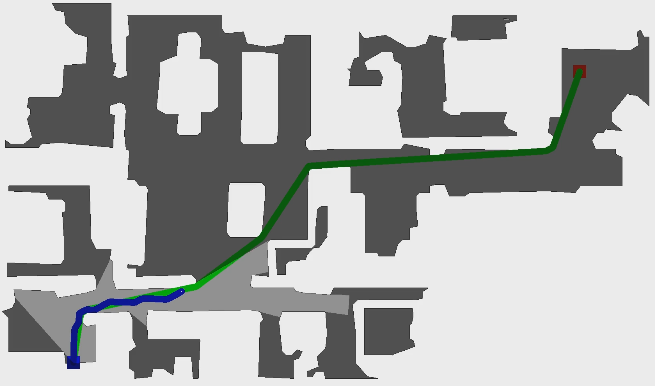
\includegraphics[width=0.6\textwidth]{imagenes/cap4/topdownmap.png}
    \caption{Mapa de un escenario de \textit{HM3D} \cite{habitatmp3d}.}
    \label{fig:chap4-topdownmap}
\end{figure}			
	
\end{itemize}

Las métricas generalmente son devueltas por el método \textit{get{\_}info} de los entornos, y son principalmente usadas durante tareas de aprendizaje por refuerzo.

\subsection{Entrenadores}

Un \textbf{entrenador} \textit{(trainer)} es una clase conteniendo los algoritmos y métodos necesarios para el entrenamiento de un agente con aprendizaje (ya sea aprendizaje por refuerzo o aprendizaje por imitación). A pesar de no estar mencionados directamente en la documentación, los entrenadores son una de las partes más esenciales del uso del simulador, al ser la principal forma de realizar el proceso de entrenamiento.

Si bien \textit{Habitat Lab} no ofrece por defecto ningún entrenador, \textit{Habitat Baselines} incluye la clase \textit{BaseTrainer} (con los métodos básicos que deben heredar los entrenadores) y \textit{BaseRLTrainer} (una subclase con métodos usados por problemas de aprendizaje por refuerzo).

Los entrenadores de aprendizaje por refuerzo deben heredar de la clase \textit{BaseRLTrainer} y ser desarrollados específicamente para el algoritmo usado, teniendo que implementar los siguientes métodos:

\begin{itemize}
	\item \textbf{\textit{save{\_}checkpoint(nombre) / load{\_}checkpoint(ruta)}:} Guardan un \textit{checkpoint} con el nombre especificado o cargan un \textit{checkpoint} con la ruta especificada, respectivamente.
	
	Para \textit{Habitat}, se suele entender un \textit{checkpoint} como un fichero comprimido conteniendo los \textbf{pesos de la red neuronal} usada durante el entrenamiento y una copia del \textbf{fichero de configuración} usado. De esta forma, es posible reanudar el entrenamiento en cualquier momento garantizando que no hay modificaciones en el entorno.
	
	\item \textbf{\textit{{\_}eval{\_}checkpoint(ruta)}:} Evalúa el rendimiento de un \textit{checkpoint} (indicado por la ruta) en el entorno. Este método es llamado desde un método superior ya implementado, \textit{eval}, que evalúa todos los \textit{checkpoints} realizados. El método se usa principalmente para elegir el \textit{checkpoint} de mayor rendimiento en el conjunto de evaluación.
	
	La forma más típica de evaluar un \textit{checkpoint} es simular uno o varios episodios enteros usando la información contenida en el \textit{checkpoint}, y posteriormente valorar las métricas del entorno para realizar una comparativa. 

	\item \textbf{\textit{train()}:} El método más importante del entrenador, \textit{train} se encarga de:
	\begin{itemize}
		\item Inicializar los modelos y estructuras de datos usadas.
		\item Simular los episodios del agente.
		\item Aplicar el algoritmo de aprendizaje, actualizando los modelos conforme son entrenados.
	\end{itemize}
	
	El entrenamiento se realiza en bucle hasta que se cumpla una de las dos condiciones de parada posibles: se alcanza el \textbf{número máximo de pasos} durante todos los episodios, o se realiza el \textbf{número de episodios} indicado. Solo se puede indicar una de las dos condiciones de parada a la vez.
	
	Por lo general, el método de entrenamiento sigue el pseudocódigo de la Figura \ref{alg:train}. Este bucle se puede modificar para añadir otras acciones que sea necesario realizar (como actualizaciones durante el episodio o registro de información).
	
	\begin{figure}[h]
\begin{algorithm}[H]
\SetAlgorithmName{Algoritmo}{algoritmo}{Lista de algoritmos}
\caption{Bucle principal de entrenamiento}
\textbf{1.} Inicializa las estructuras de datos necesarias para el entrenamiento, los contadores globales de pasos $num\_steps\_done$ y actualizaciones $num\_updates\_done$, y los modelos a entrenar.\\
\textbf{2.} Mientras no se cumpla la condición de parada (número máximo de pasos o número de actualizaciones):\\
\Indp \textbf{2.1.} Prepara el escenario (a través del método \textit{reset} del entorno)\\
\textbf{2.2.} Mientras no haya finalizado el episodio:\\
\Indp \textbf{2.2.1.} El agente percibe el estado del escenario a través de los sensores.\\
\textbf{2.2.2.} El agente procesa el estado, actualizando su modelo si es necesario, y eligiendo una acción.\\
\textbf{2.2.3.} El agente aplica la acción (a través del método \textit{step} del entorno).\\
\textbf{2.2.4.} Incrementa el contador global de pasos $num\_steps\_done$.\\
\Indm \textbf{2.3.} Actualiza el modelo.\\
\textbf{2.4.} Si es necesario, guarda un \textit{checkpoint} del estado actual del modelo.\\
\textbf{2.5.} Incrementa el contador global de actualizaciones $num\_updates\_done$.
\end{algorithm}
\hrule
\caption{Pseudocódigo del bucle principal de entrenamiento.}
\label{alg:train}
\end{figure}
\end{itemize}


\textit{BaseRLTrainer} además incluye varios métodos ya implementados para facilitar el desarrollo del entrenamiento y la comprobación de las condiciones:

\begin{itemize}
	\item \textbf{\textit{is{\_}done()}:} Devuelve un valor booleano \textbf{verdadero} si se ha cumplido la condición de parada (ya sea número de pasos o de episodios), o \textbf{falso} en otro caso. Este método se usa para controlar el bucle general de entrenamiento.
	\item \textbf{\textit{should{\_}checkpoint()}:} Devuelve un valor booleano \textbf{verdadero} si es necesario realizar un \textit{checkpoint}, o \textbf{falso} en otro caso.
	
	Este método calcula automáticamente el porcentaje de entrenamiento realizado, y si es necesario realizar un \textit{checkpoint} en base a dicho porcentaje (a partir del número de \textit{checkpoints} que se ha especificado en el fichero de configuración).
\end{itemize}

En el trabajo se ha implementado un entrenador personalizado (\textit{ReactiveNavigationTrainer}) como subclase de \textit{BaseRLTrainer}, implementando un algoritmo de aprendizaje por refuerzo via \textit{Deep Q-Learning}.

\subsection{Agentes}

Un \textbf{agente} (\textit{agente}) es un contenedor para los modelos entrenados, diseñado para ser usado con los \textit{benchmarks} de \textit{Habitat}.

Los agentes deben heredar de la clase \textit{Agent}, e implementar los dos siguientes métodos:

\begin{itemize}
	\item \textbf{\textit{reset()}:} Prepara al agente para el inicio de un nuevo episodio.
	\item \textbf{\textit{act(observaciones)}:} A partir de las observaciones, el agente debe devolver una acción a realizar en forma de diccionario $\{action="accion\_elegida"\}$.
\end{itemize}

Estos métodos son llamados automáticamente por el entorno contenido en el \textit{benchmark}.

\textit{Habitat Baselines} ofrece algunos agentes preconstruidos (principalmente agentes heurísticos para funcionar como \textit{benchmark} y un agente de aprendizaje aplicando \textit{PPO}). En este trabajo se ha diseñado un agente propio (\textit{ReactiveNavigationAgent}) para evaluar el rendimiento de la propuesta.

En contra de lo que pueda dar a entender el nombre del concepto, los agentes no tienen ninguna relación con los agentes físicos simulados, y su uso se limita exclusivamente a \textit{benchmarks}.

\subsection{\textit{Benchmarks}}

\textit{Habitat} ofrece por defecto un \textit{benchmark} con el que se puede evaluar el rendimiento de los agentes ya entrenados. El benchmark recibe como entrada un agente (definido previamente) y el número de episodios que se quiere evaluar (por defecto todos los posibles), y se encarga de:

\begin{itemize}
	\item Crear y gestionar el entorno (usando un entorno \textit{Env}).
	\item Simular internamente los episodios, usando los métodos del entorno y del agente.
	\item Obtener las métricas de cada episodio realizado.
\end{itemize}

El \textit{benchmark} devuelve como resultado final el valor medio de cada métrica tras todos los episodios evaluados, para poder ser analizado y comparado con otros agentes.

\subsection{Ficheros de configuración}

\textit{Habitat} usa un \textbf{fichero de configuración} para cargar todos los parámetros necesarios para su funcionamiento. Este fichero es, junto a los entrenadores, una de las partes más importantes del uso del simulador, pese a no estar recogida en la documentación.

Los ficheros de configuración son documentos en formato \textit{YAML} \cite{yaml} divididos en bloques. Dentro de cada bloque hay pares de clave - valor que se corresponden al parámetro a configurar (clave) y el valor asignado a ese parámetro (valor).

Los principales bloques del fichero de configuración son:

\begin{itemize}
	\item \textbf{ENVIRONMENT:} En este bloque se incluyen parámetros relativos al entorno, incluyendo la forma en la que se ordenan los episodios o las duraciones máximas de éstos. Algunas de las claves principales de éste bloque son:
	
	\begin{itemize}
		\item \textbf{MAX{\_}EPISODE{\_}STEPS:} Pasos máximos que puede dar un agente en un episodio. Si se supera este valor, el episodio se finaliza inmediatamente.
		\item \textbf{MAX{\_}EPISODE{\_}SECONDS:} Duración máxima del episodio en segundos. Si se supera este valor, el episodio se finaliza inmediatamente.
	\end{itemize}
	
	\item \textbf{SIMULATOR:} En este bloque se incluyen parámetros relativos al simulador y al agente, como los sensores a usar o los parámetros de éstos. Algunas de las claves principales de este bloque son:
	
	\begin{itemize}
		\item \textbf{AGENT{\_}0:} Sub-bloque donde se encuentra la información sobre el agente. Su clave más importante es \textbf{SENSORS}, donde se indica en una lista (entre corchetes) los sensores a usar.
		\item \textbf{RGB{\_}SENSOR / DEPTH{\_}SENSOR:} Sub-bloques donde se especifican los parámetros de los sensores, \textbf{WIDTH} (anchura en píxeles de la imagen devuelta por el sensor) y \textbf{HEIGHT} (altura en píxeles). El resto de sensores se pueden configurar de una forma similar.
	\end{itemize}
	
	\item \textbf{DATASET:} Contiene información sobre el conjunto de datos a utilizar. Algunas de las claves principales de este bloque son:
	\begin{itemize}
		\item \textbf{TYPE:} Tipo de conjunto de datos a utilizar. Este tipo se debe corresponder con el tipo de tarea a realizar.
		\item \textbf{DATA{\_}PATH:} Ruta a los ficheros del conjunto de datos a utilizar. Se puede usar la palabra $\{split\}$ para indicar una sección de la ruta que se sustituye por el valor de la variable \textbf{SPLIT}.
		\item \textbf{SPLIT:} Partición del conjunto de datos a utilizar. Por defecto, las particiones son \textbf{train} (entrenamiento) y \textbf{val} (validación).
	\end{itemize}
	
	\item \textbf{TASK:} Contiene información sobre la tarea a realizar y las métricas a utilizar. Algunas de las claves principales de este bloque son:
	\begin{itemize}
		\item \textbf{SENSORS:} Lista de métricas a usar para la valoración de la tarea. Estas métricas pueden personalizarse en sub-bloques, de forma similar a la configuración de los sensores.
		\item \textbf{SUCCESS{\_}DISTANCE:} Distancia (en metros) a la que tiene que estar el agente de la meta para que se considere que el episodio se ha completado con éxito.
	\end{itemize}
	
	\item \textbf{RL:} Contiene información relacionada con el aprendizaje por refuerzo, para ser usada por los entrenadores. Esta sección es opcional y no tiene una estructura fija, pudiendo añadir las claves deseadas para ser leídas posteriormente.
	
	\item \textbf{Claves sin bloque:} Se pueden indicar claves fuera del resto de bloques, quedando a la altura de la raíz. Estas claves en general están relacionadas con configuraciones para los procesos de entrenamiento y registro de datos, siendo algunas de las principales:
	\begin{itemize}
		\item \textbf{BASE{\_}TASK{\_}CONFIG{\_}PATH:} Ruta al fichero de configuración base. Si se especifica este valor, los valores contenidos en este fichero se fusionarán con los del fichero indicado. Permite crear una configuración base sobre la que crear variaciones.
		\item \textbf{TRAINER{\_}NAME / ENV{\_}NAME:} Identificador del entrenador o del entorno a utilizar, respectivamente. Estos identificadores se usan para obtener la clase adecuada del registro (como se verá después).
		\item \textbf{TOTAL{\_}NUM{\_}STEPS / NUM{\_}UPDATES:} Número máximo de pasos o actualizaciones a realizar durante el entrenamiento. El entrenamiento dura hasta que se alcanza uno de estos valores. Solo puede aparecer una de las dos claves en el fichero.
		\item \textbf{NUM{\_}CHECKPOINTS:} Número total de \textit{checkpoints} a realizar durante el proceso de entrenamiento.
		\item \textbf{CHECKPOINT{\_}FOLDER:} Carpeta en la que se almacenarán los \textit{checkpoints} realizados.
	\end{itemize}
	
	Existen más claves dentro de esta categoría, pudiendo observarse en los ficheros de configuración de ejemplo.
\end{itemize}

Se puede ver un ejemplo de un fichero de configuración para una tarea de navegación usando \textit{Gibson} en la Figura \ref{fig:chap4-conf}. Además, se pueden ver los ficheros de configuración desarrollados (documentados en inglés) en el Anexo B (Ficheros de configuración).

\begin{figure}[!ht]
\centering
\begin{lstlisting}[language=yaml]
ENVIRONMENT:
  MAX_EPISODE_STEPS: 500
SIMULATOR:
  AGENT_0:
    SENSORS: ['RGB_SENSOR']
  HABITAT_SIM_V0:
    GPU_DEVICE_ID: 0
  RGB_SENSOR:
    WIDTH: 256
    HEIGHT: 256
  DEPTH_SENSOR:
    WIDTH: 256
    HEIGHT: 256
TASK:
  TYPE: Nav-v0
  SUCCESS_DISTANCE: 0.2

  SENSORS: ['POINTGOAL_WITH_GPS_COMPASS_SENSOR']
  POINTGOAL_WITH_GPS_COMPASS_SENSOR:
    GOAL_FORMAT: "POLAR"
    DIMENSIONALITY: 2
  GOAL_SENSOR_UUID: pointgoal_with_gps_compass

  MEASUREMENTS: ['DISTANCE_TO_GOAL', 'SUCCESS', 'SPL']
  SUCCESS:
    SUCCESS_DISTANCE: 0.2

DATASET:
  TYPE: PointNav-v1
  SPLIT: train
  DATA_PATH: data/datasets/pointnav/gibson/v1/{split}/{split}.json.gz
\end{lstlisting}
\caption{Fichero de configuración por defecto para tareas de navegación usando \textit{Gibson}.}
\label{fig:chap4-conf}
\end{figure}

El simulador no trabaja directamente con el fichero de configuración, sino que primero convierte el contenido del fichero a un objeto de la clase \textit{Config}. Este objeto contiene todos los valores del fichero en forma de diccionario, y se puede obtener de la siguiente forma:

\begin{itemize}
	\item \textbf{Método \textit{get{\_}config(ruta)} de \textit{Habitat Lab}:} Este método (disponible en el fichero \textit{habitat/config/default.py}) genera una instancia de \textit{Config} a partir de una serie de valores por defecto y los valores indicados en el fichero de configuración. Es recomendable usar este método para configuraciones relacionadas con \textit{benchmarks}.
	\item \textbf{Método \textit{get{\_}config(ruta)} de \textit{Habitat Baselines}:} Este método se diferencia del anterior en tres puntos:
	\begin{itemize}
		\item Incluye valores por defecto de aprendizaje por refuerzo.
		\item Es capaz de cargar los valores de otro fichero de configuración (indicado con la clave \textit{BASE{\_}TASK{\_}CONFIG{\_}PATH}.
		\item Almacena los valores de los cuatro bloques principales (\textit{ENVIRONMENT, SIMULATOR, DATASET} y \textit{TASK}) bajo un nuevo bloque llamado \textit{TASK{\_}CONFIG}.
	\end{itemize}	 
	Es recomendable usar este método para configuraciones de entrenadores.
\end{itemize}

\subsection{Registros}

Un \textbf{registro} (\textit{registry}) es un contenedor global y central de información, en el que se almacenan pares de clave y clase asociada a la clave. Estos registros sirven para poder instanciar las clases apropiadas (de simulador, tarea, entorno...) a partir de sus identificadores, siendo especialmente útil para cargar las clases indicadas en el fichero de configuración.

Los registros funcionan usando \textbf{decoradores}, funciones que se llaman durante la definición de las clases y que las registran para poder acceder a ellas posteriormente desde cualquier punto del código.

Por defecto, \textit{Habitat} incluye dos registros, cada uno almacenando información distinta:

\begin{itemize}
	\item \textbf{Registro \textit{Registry} de \textit{Habitat Lab}:} El registro principal en el que se incluye información sobre:
	\begin{itemize}
		\item \textbf{Tareas}, usando el decorador \textit{@registry.register{\_}task}.
		\item \textbf{Acciones}, usando el decorador \textit{@registry.register{\_}task{\_}action}.
		\item \textbf{Simuladores}, usando el decorador \textit{@registry.register{\_}simulator}.
		\item \textbf{Sensores}, usando el decorador \textit{@registry.register{\_}sensor}.
		\item \textbf{Métricas}, usando el decorador \textit{@registry.register{\_}measure}.
		\item \textbf{Conjuntos de datos}, usando el decorador \textit{@registry.register{\_}dataset}.
	\end{itemize}
	\item \textbf{Registro \textit{BaselineRegistry} de \textit{Habitat Baselines}:} Un registro adicional pensado para almacenar las clases creadas por el usuario, incluye información sobre:
	\begin{itemize}
		\item \textbf{Entornos}, usando el decorador \textit{@baseline{\_}registry.register{\_}env}.
				\item \textbf{Entrenadores}, usando el decorador \textit{@baseline{\_}registry.register{\_}trainer}.
				\item \textbf{Políticas de acciones}, usando el decorador \textit{@baseline{\_}registry.register{\_}policy}.
	\end{itemize}
\end{itemize}

\section{Instalación de \textit{Habitat}}

El proceso de instalación de \textit{Habitat} puede resultar complicado debido a la gran cantidad de componentes y versiones específicas necesarias. Por eso, en esta sección se indican los pasos necesarios para instalar el entorno de \textit{Habitat}, remarcando los requisitos de versiones necesarios para el funcionamiento adecuado.

\subsection{Requisitos}

El entorno de \textit{Habitat} requiere versiones específicas de 

\begin{itemize}
	\item \textbf{Python:} Versión superior a \textit{3.6.0} (recomendable usar \textit{3.6.10}).
	\item \textbf{cmake:} Versión superior a \textit{3.10} (recomendable usar \textit{3.14.0}).
	\item \textbf{Sistema operativo:} Si bien \textit{Habitat Sim} incluye soporte para Windows, es recomendable usar alguna distribución de \textit{Linux} con soporte para \textit{CUDA}. En este trabajo se ha utilizado \textbf{Ubuntu 20.04}.
	\item \textbf{Tarjeta gráfica:} En caso de ser necesaria, se necesita una tarjeta gráfica de \textit{nVidia} que ofrezca soporte para \textit{CUDA}.
	\item \textbf{CUDA:} Se ha usado la versión \textit{11.0} en el trabajo realizado, aunque es posible que dependiendo de la configuración se necesite otra.
\end{itemize}

Además, la instalación de \textit{Habitat Lab} y \textit{Habitat Baselines} instala versiones concretas de diversas librerías de \textit{Python}, por lo que es recomendable instalar \textit{Habitat} en un entorno propio de \textit{Conda} para evitar problemas de compatibilidad. 

\subsection{Proceso de instalación}

Si bien es posible utilizar \textit{dockers} para instalar el entorno del simulador, es recomendable realizar la instalación directamente para garantizar acceso a las actualizaciones. El proceso de instalación en distribuciones de \textit{Linux} se puede dividir en tres pasos principales:

\begin{enumerate}
	\item \textbf{Instalación de CUDA:} Para el uso de \textit{Habitat} y para el entrenamiento adecuado de redes neuronales, es necesaria una instalación correcta y completa de CUDA. Para esto, es necesario:
	\begin{enumerate}
		\item Tener \textit{drivers} \textbf{oficiales} de \textit{nVidia}, actualizados a la versión más moderna. No es necesaria una versión concreta del \textit{driver}.
		\item Instalar \textbf{CUDA}. La guía oficial de instalación en \textit{Linux}\footnote{\url{https://docs.nvidia.com/cuda/cuda-installation-guide-linux/index.html}} incluye los pasos a seguir, mientras que la página de descarga\footnote{\url{https://developer.nvidia.com/cuda-downloads}} ofrece las instrucciones para descargar e instalar CUDA.
		
		Es recomendable seguir los pasos de pre-instalación y post-instalación indicados en la guía oficial, pero seguir los pasos de la página de descarga para la instalación.
		
		\item Instalar \textbf{cuDNN}. La guia oficial de instalación en \textit{Linux}\footnote{\url{https://docs.nvidia.com/deeplearning/cudnn/install-guide/index.html}} incluye los pasos necesarios para instalar cuDNN. Es importante comprobar que las versiones de CUDA y cuDNN instaladas sean compatibles entre sí.
		
		Es necesaria una cuenta de desarrollador de \textit{nVidia} para la descarga de cuDNN.
	\end{enumerate}
	\item \textbf{Instalación de \textit{Habitat Sim}:} La instalación de \textit{Habitat Sim} se hace a través del repositorio de paquetes \textit{Conda}. Además, como se ha comentado previamente, es recomendable crear un entorno propio de \textit{Conda} para evitar problemas de compatibilidades. 
	
	Contando con una instalación válida de \textit{Conda}, los siguientes comandos en una terminal crean un entorno con las versiones adecuadas de \textit{Python} y \textit{cMake} e instalan \textit{Habitat Sim}:

\begin{lstlisting}[language=bash]
# Crea el entorno de Conda con las versiones adecuadas de Python y cMake
conda create -n habitat python=3.6 cmake=3.14.0
# Inicializa el entorno creado
conda activate habitat
# Instala el simulador con soporte para fisicas (withbullet)
conda install habitat-sim withbullet -c conda-forge -c aihabitat
\end{lstlisting}	
	
	\item \textbf{Instalación de \textit{Habitat Lab} y \textit{Habitat Baselines}:} Ya con el simulador instalado, el último paso es instalar la librería \textit{Habitat Lab}. Si bien \textit{Habitat Baselines} es opcional, es muy recomendable su instalación por las utilidades adicionales que ofrece. Los siguientes comandos en una terminal instalan \textit{Habitat Lab} y \textit{Habitat Baselines}:
	
\begin{lstlisting}[language=bash]
# Descarga la version mas reciente del repositorio de Habitat Lab
# El repositorio se descarga en la carpeta actual
git clone --branch stable https://github.com/facebookresearch/habitat-lab.git
# Accede al repositorio descargado
cd habitat-lab
# Instala todos los paquetes de Python necesarios
# Es recomendable realizar la instalacion en el mismo entorno que Habitat Sim
# para evitar incompatibilidades
pip install -r requirements.txt
# Instala Habitat Lab y Habitat Baselines
python setup.py develop --all
\end{lstlisting}	
\end{enumerate}

Para comprobar que la instalación se ha realizado correctamente, \textit{Habitat Lab} ofrece el fichero \textit{examples/example.py}. Si no ha habido ningún problema en la instalación, al ejecutar el fichero se realizará una simulación con un agente de ejemplo ofrecido por defecto por \textit{Habitat}, imprimiendo en la terminal el número de pasos realizado.
